% !TEX root = ../main.tex
\section{实验\chinese{section}}
\subsection{实验题目}
数字IO实验
\subsection{实验目的}
端口中断应用:检测P2.6和P2.7的按键输入,按下时(下跳沿)进端口中断,在中断服务程序内检测相应标志位,若P2.6口按键按下,P4.1输出高电平;若P2.7口按键按下,P4.1输出低电平,实现对应LED的状态控制。
\subsection{实验仪器和设备}
计算机、开发板、示波器、信号源、电源、Code Composer Studio v5、串口调试助手等。
\subsection{实验步骤}
\begin{lstlisting}[language=C]
/****************************************
KEY1-->|P2.6 P4.2|-->LED_GREEN
KEY2-->|P2.7 P4.1|-->LED_YELLOW
     --|RST      |
****************************************/
\end{lstlisting}
\par\indent 关闭看门狗,打开总中断。并设置P2.6和P2.7为输入引脚,设置中断使能并设置为下降沿触发。主程序内执行一个死循环。这样,当检测到按键按下(一个低电平边沿),触发中断,并控制LED点亮。按键使用软件延时,实现防抖功能。
\subsection{程序清单}
\lstinputlisting{src/code/IO.c}
\subsection{实验结果记录与分析}
\begin{figure}[htbp]
	\centering
	\begin{minipage}[htbp]{7.5cm}
		\centering
		\caption{IO,按下USER\_1}
		\label{IO1}
		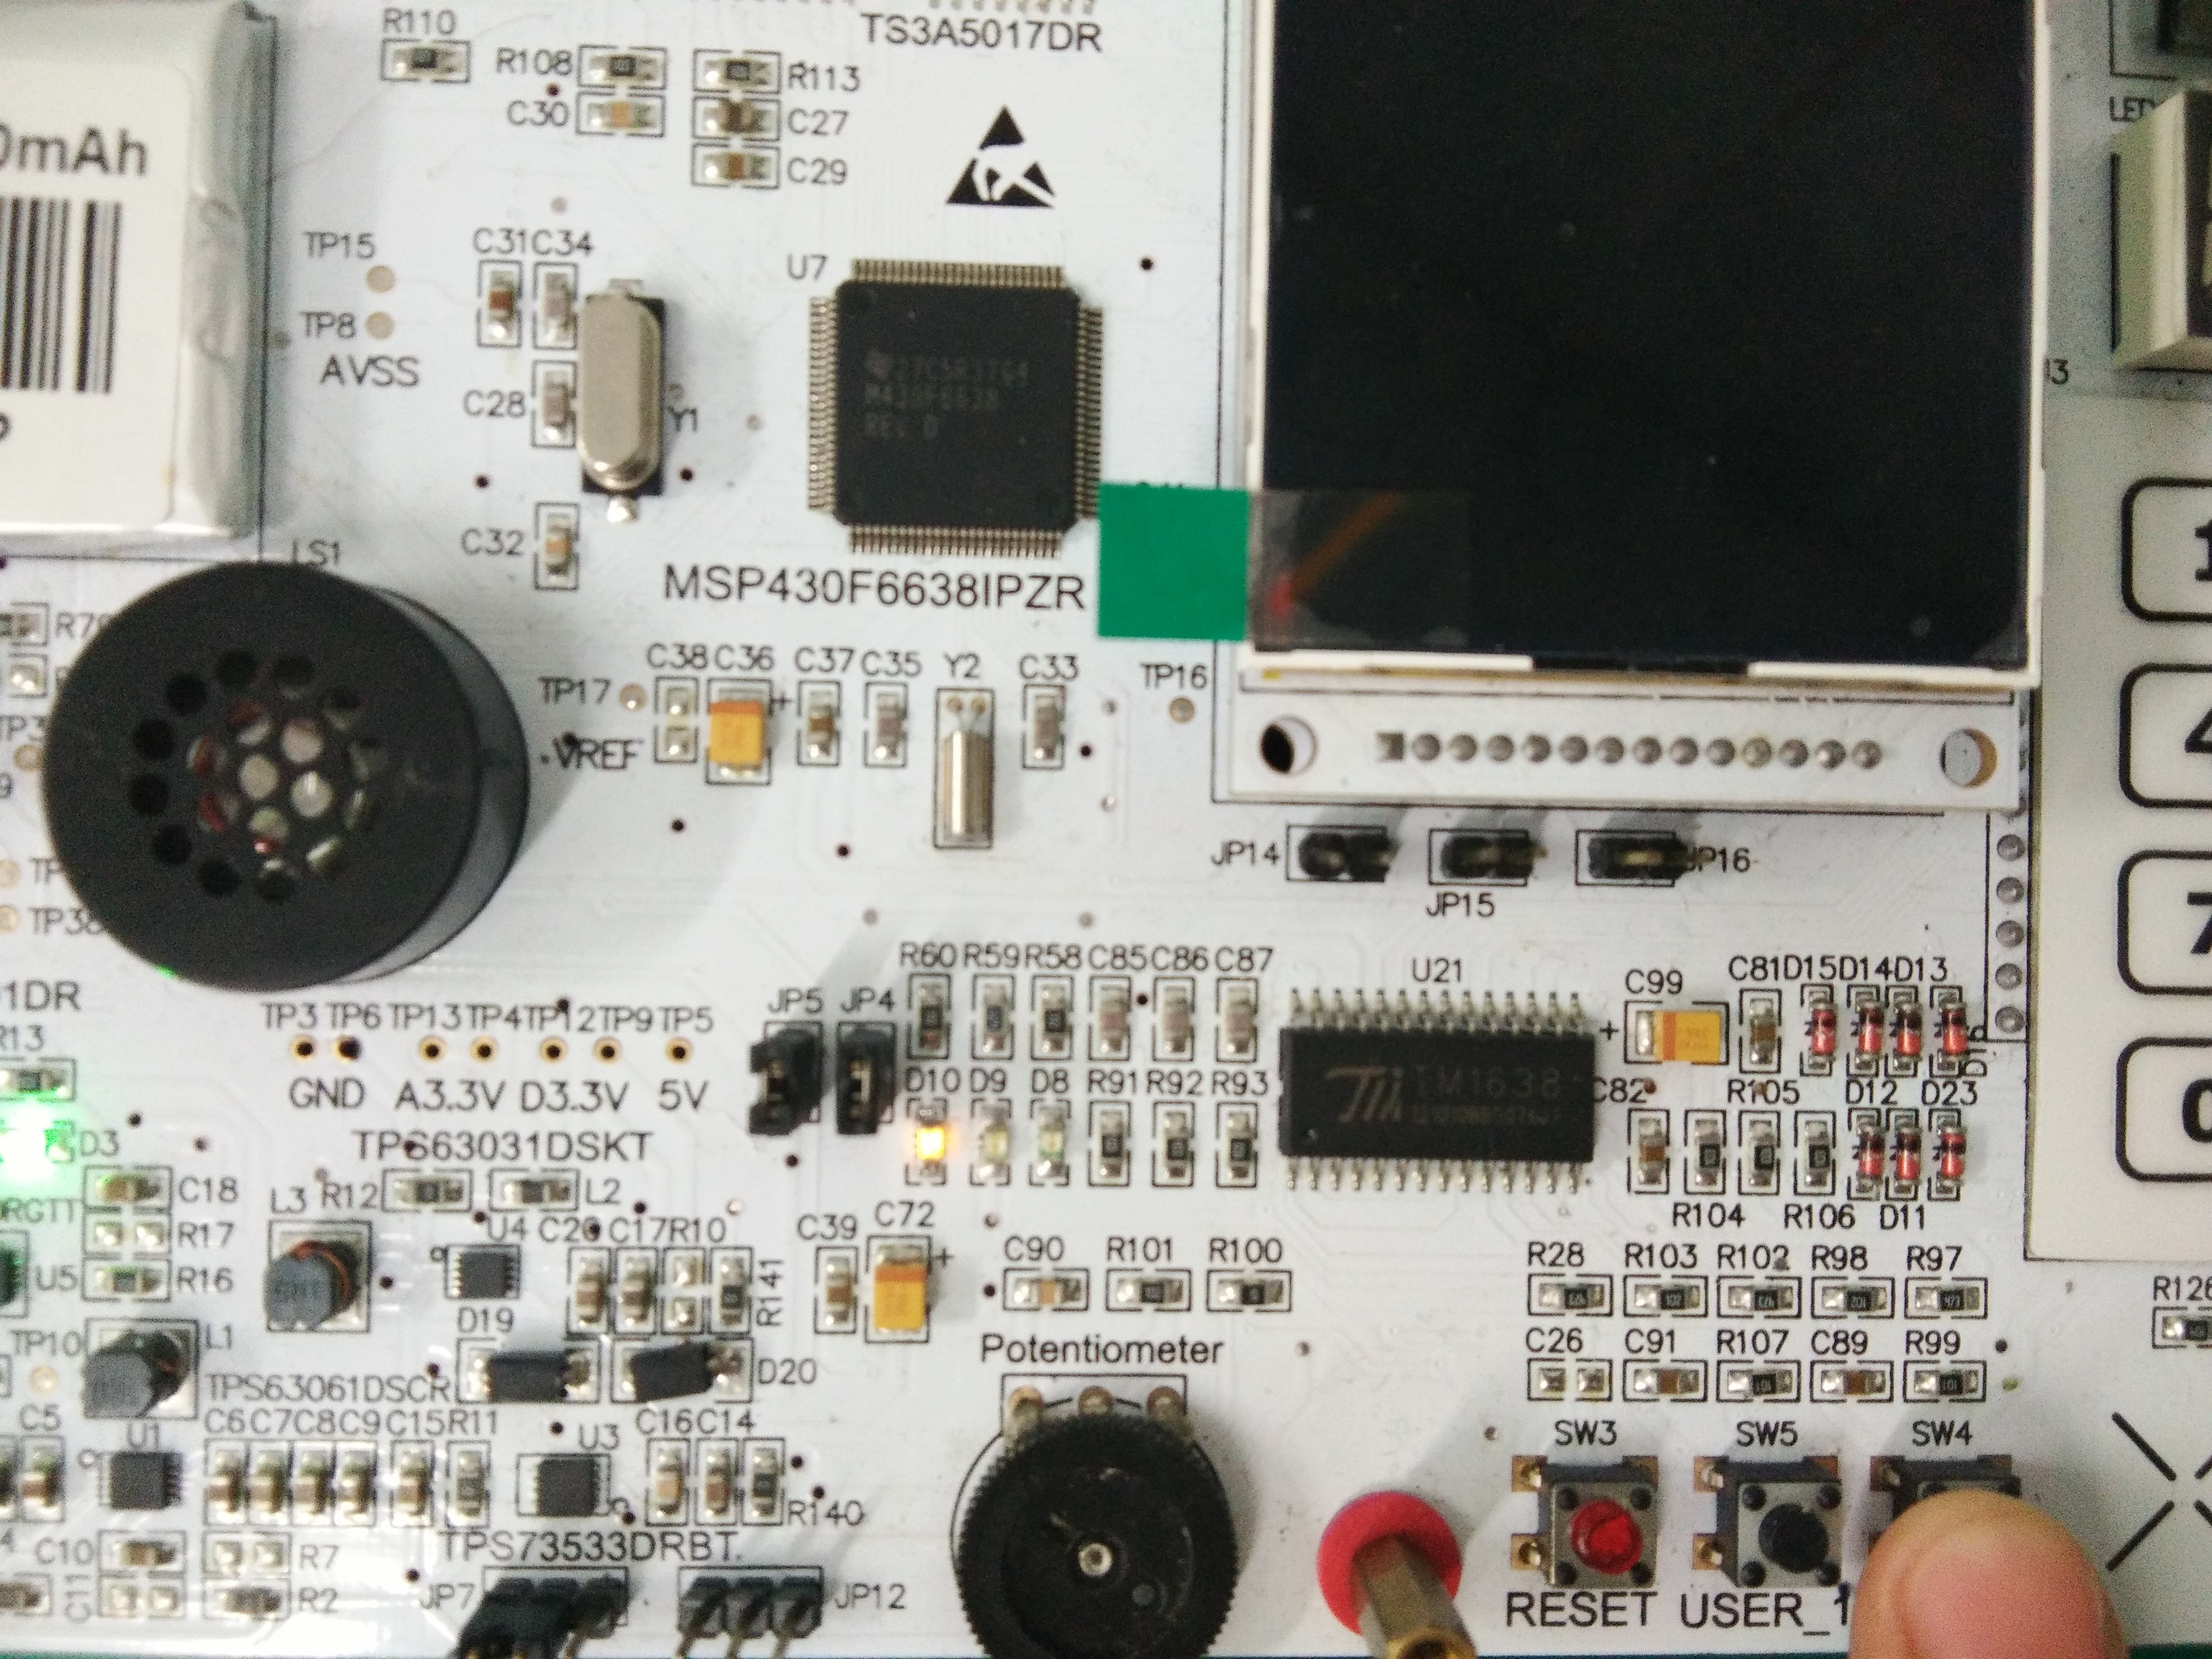
\includegraphics[width=7.5cm]{bitmap/jpg/IO1.jpg}
	\end{minipage}
	\begin{minipage}[htbp]{7.5cm}
		\centering
		\caption{IO,按下USER\_2}
		\label{IO2}
		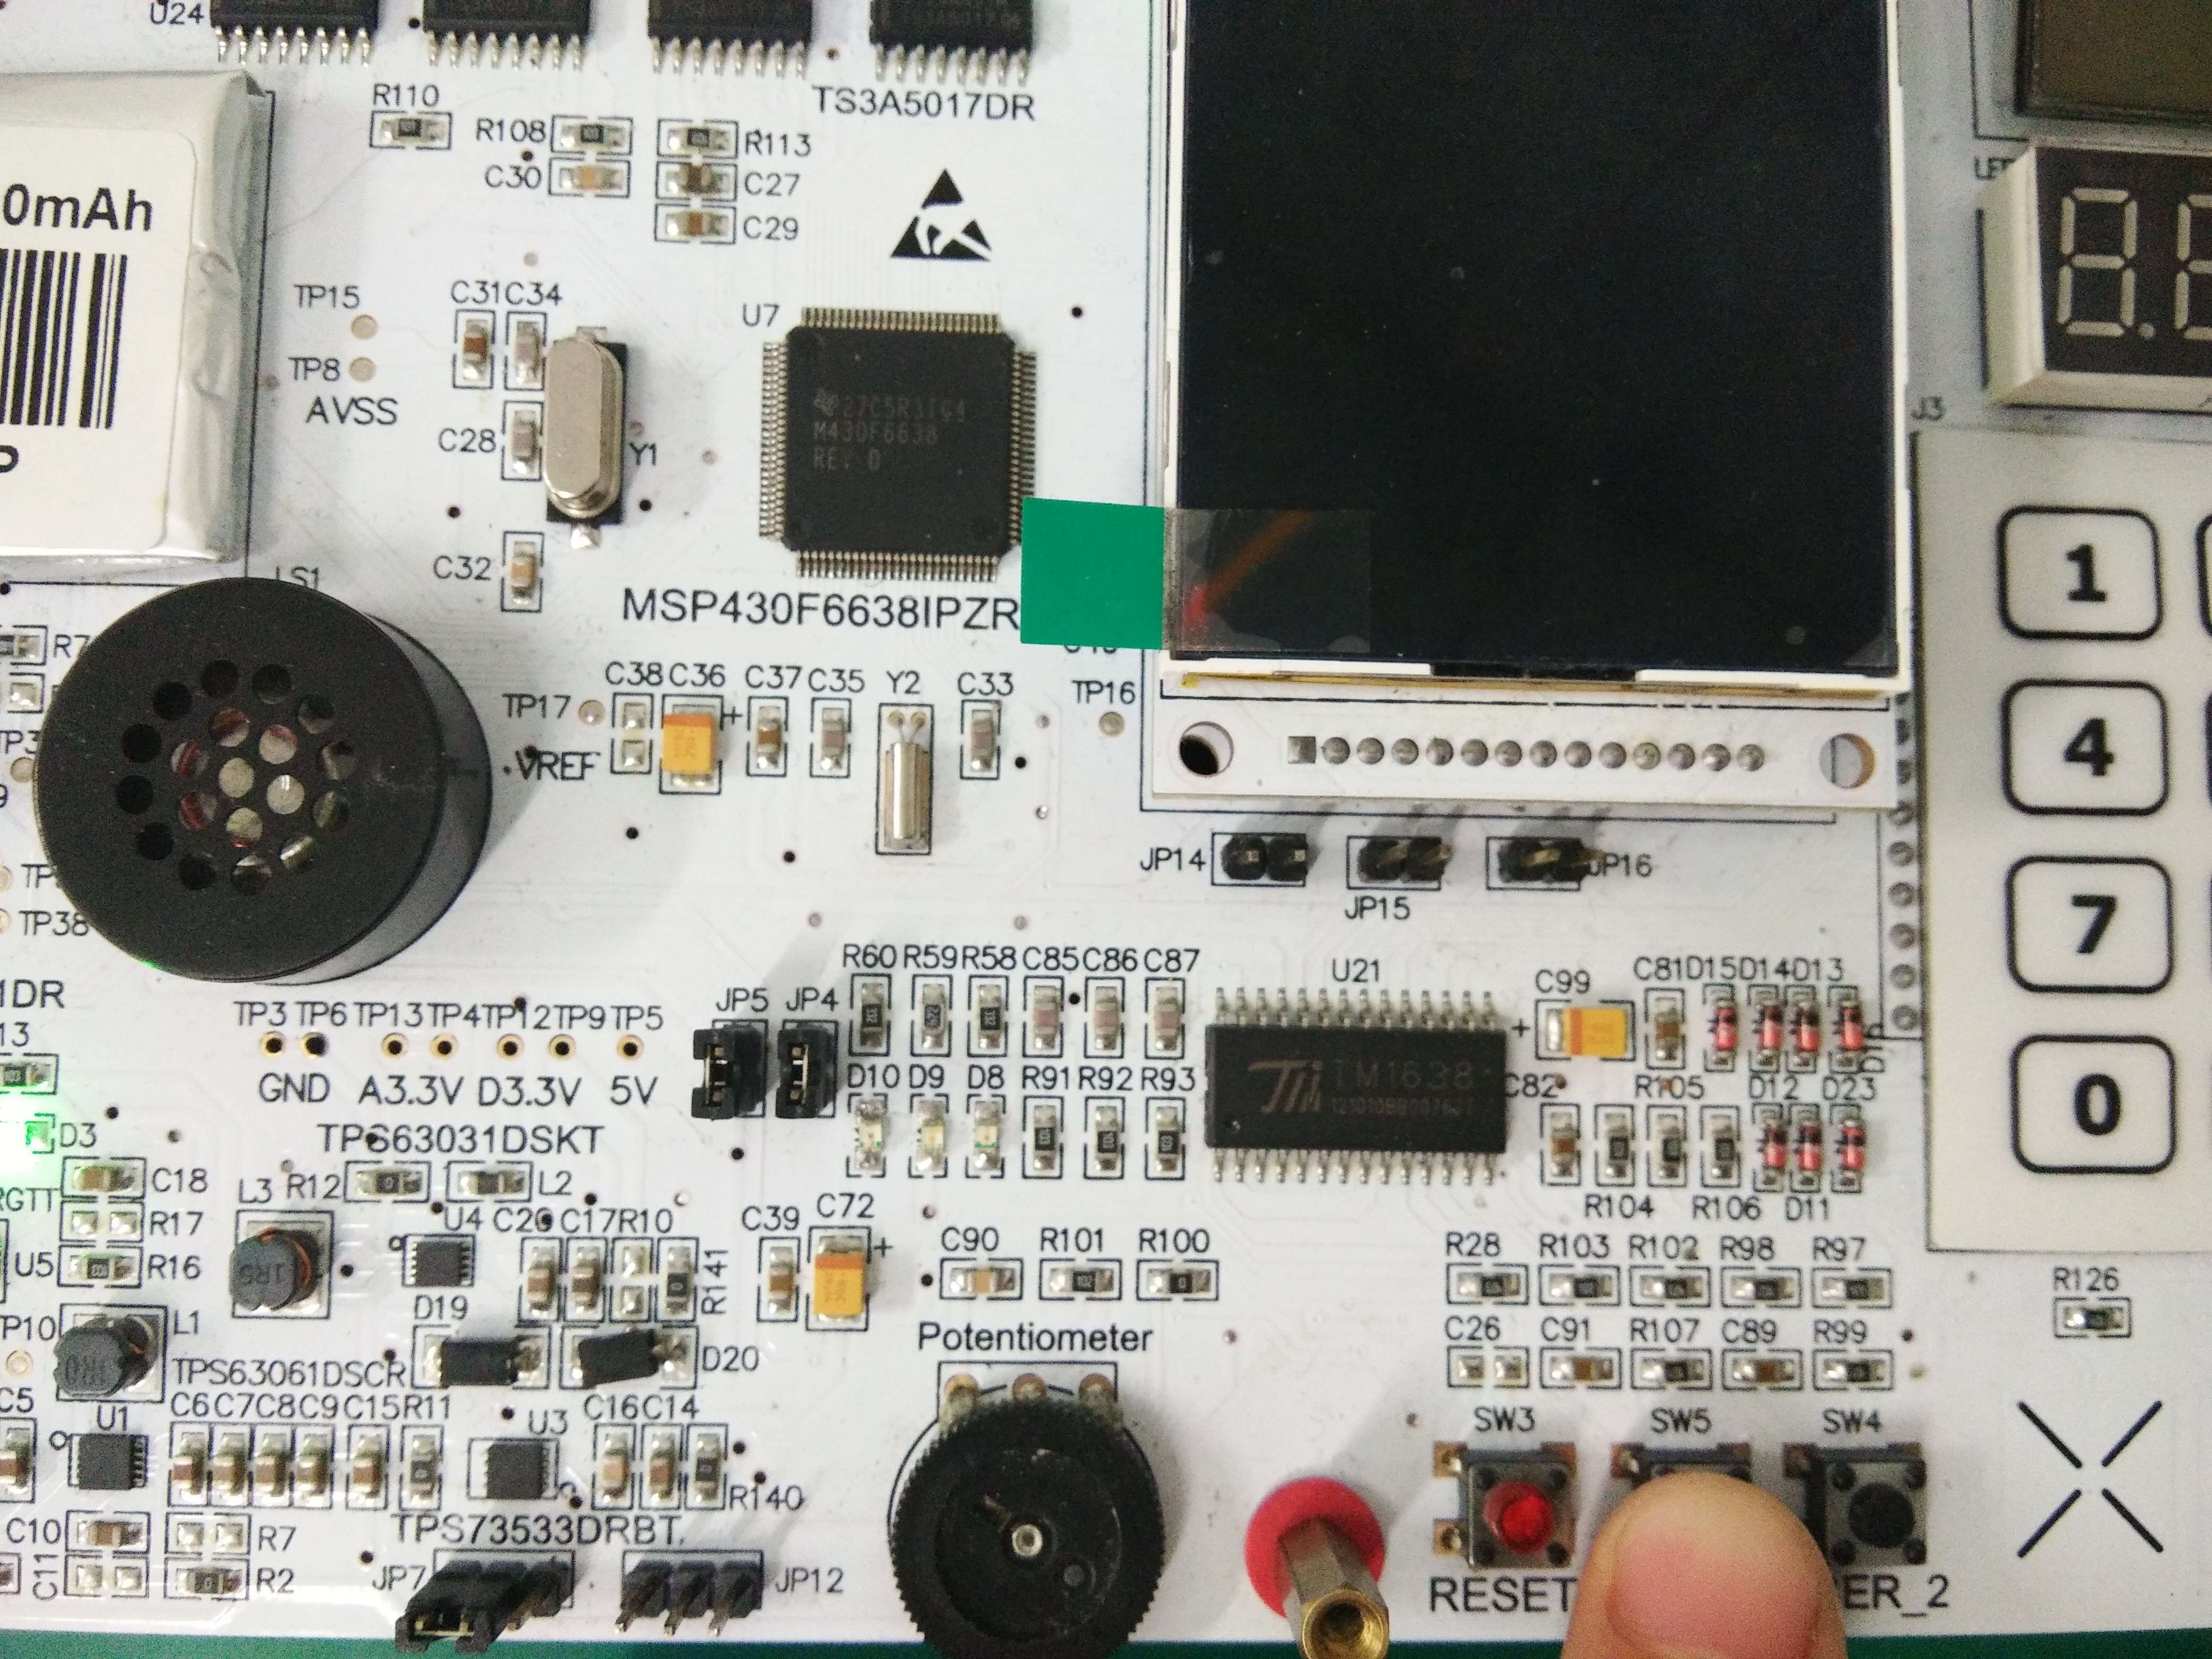
\includegraphics[width=7.5cm]{bitmap/jpg/IO2.jpg}
	\end{minipage}
\end{figure}
\subsection{遇到的问题与解决方法}
\begin{enumerate}
	\item 在写多源中断的程序时注意到一个有趣的问题。P1、P2和TimerA、ADC12都是多源中断,都需要在中断服务程序中手动清除IFG和查询具体是哪个中断源触发中断。但例程对它们的处理却截然不同。对于P1和P2,处理方式是访问IFG,然后IFG清0,而TimerA和ADC12却是访问IV,然后IFG不用清0。之后查询了用户手册才发现这2种方式是等效的。只不过P1和P2的IFG都在1个控制字上,方便按位判断0、1。但规范的方法还是应该访问IV。而且访问IV后对应的IFG会自动清0,省事一点。另外IV里面定义了宏,不容易写错。
\end{enumerate}

